\section{Clase 5 - Pr\'actica 3 (Ecuaciones diferenciales - Problema de valores de contorno)}

\subsection{Diferencias finitas}

Partimos de un problema de valores de contorno

$$ 
	\begin{cases}
        u''(x) = p(x)u'(x) + q(x)u(x) + f(x)\\
        u(a) = \alpha,\ u(b) = \beta \\
    \end{cases}
$$

Buscamos $(u_{0}, \cdots, u_{N})$ de forma tal que $u_{j} \approx u(x_{j}),\ 1 \leq j \leq N - 1$.\\

\underline{Teorema}: Dada la ecuaci\'on de segundo orden $u''(x) = p(x)u'(x) + q(x)u(x) + f(x)$, con $a \leq x \leq b$ y valores en la frontera $u(a) = \alpha,\ u(b) = \beta$. Si $p, q, f$ son continuas en $[a, b]$ y $q > 0$, entonces el problema tiene soluci\'on \'unica.\\

Sea $N \in \mathbb{N}$, tomamos un paso $h = \frac{b - a}{N}$ y consideramos los puntos $x_{j} = a + jh$ con $j = 0, \cdots, N$ (notar que $x_{0} = a$ y $x_{N} = b$). Definimos $u_{0} = \alpha,\ u_{N} = \beta$ y aproximamos las derivadas de $u$.\\

\subsection{Discretizaciones usuales de $u'$}

$$\text{FORWARD}\ \ \ u'(x) \approx \frac{u(x_{j + 1}) - u(x_{j})}{h}$$

$$\text{BACKWARD}\ \ \ u'(x) \approx \frac{u(x_{j}) - u(x_{j - 1})}{h}$$

$$\text{CENTRADA}\ \ \ u'(x) \approx \frac{u(x_{j + 1}) - u(x_{j - 1})}{2h}$$

\subsection{Discretizaci\'on usual de $u''$}

$$u(x + h) = u(x) + hu'(x) + \frac{h^{2}}{2!}u''(x) + \frac{h^{3}}{3!}u'''(x) + \frac{h^{4}}{4!}u^{IV}(\zeta_{1})$$

$$u(x - h) = u(x) - hu'(x) + \frac{h^{2}}{2!}u''(x) - \frac{h^{3}}{3!}u'''(x) + \frac{h^{4}}{4!}u^{IV}(\zeta_{2})$$

$$\Rightarrow u(x + h) + u(x - h) = 2u(x) + h^{2}u''(x) + \frac{h^{4}}{4!}(u^{IV}(\zeta_{1}) + u^{IV}(\zeta_{2}))$$

$$u''(x) = \frac{u(x + h) - 2u(x) + u(x - h)}{h^{2}} - \frac{h^{2}}{4!}(u^{IV}(\zeta_{1}) + u^{IV}(\zeta_{2})) = \frac{u(x + h) - 2u(x) + u(x - h)}{h^{2}} - \mathcal{O}(h^{2})$$

Llamamos $p_{j} = p(x_{j}),\ q_{j} = q(x_{j}),\ f_{j} = f(x_{j})$ y usando diferencias centradas proponemos:

$$\frac{u_{j + 1} - 2u_{j} + u_{j - 1}}{h^{2}} = p_{j}\frac{u_{j + 1} - u_{j - 1}}{2h} + q_{j}u_{j} + f_{j}$$

Multiplicando por $h^{2}$ y reagrupando:

$$u_{j + 1} - 2u_{j} + u_{j - 1} - \frac{1}{2}hp_{j}(u_{j + 1} - u_{j - 1}) - h^{2}q_{j}u_{j} = h^{2}f_{j}$$

$$\bigg(1 + \frac{1}{2}hp_{j}\bigg)u_{j - 1} - (2 + h^{2}q_{j})u_{j} + \bigg(1 - \frac{1}{2}hp_{j}\bigg)u_{j + 1} = h^{2}f_{j}$$

\begin{itemize}
	\item $j = 1:\ -(2 + h^{2}q_{1})u_{1} + \bigg(1 - \frac{1}{2}hp_{1}\bigg)u_{2} = h^{2}f_{1} - \bigg(1 + \frac{1}{2}hp_{1} \bigg)u_{0},\ u_{0} = \alpha$
	
	\item $2\leq j \leq N - 2:\ \bigg(1 + \frac{1}{2}hp_{j}\bigg)u_{j - 1} - (2 + h^{2}q_{j})u_{j} + \bigg(1 - \frac{1}{2}hp_{j}\bigg)u_{j + 1} = h^{2}f_{j}$
	
	\item $j = N - 1:\ \bigg(1 + \frac{h}{2}p_{N - 1}\bigg)u_{N - 2} - (2 + h^{2}q_{N - 1})u_{N - 1} = h^{2}f_{N - 1} - \bigg(1 - \frac{h}{2}p_{N - 1}\bigg)u_{N},\ u_{N} = \beta$
\end{itemize}

En forma matricial: $A_{h}u_{h} = b_{h}$,

$$
    \begin{pmatrix}
        -(2 + h^{2}q_{1}) & (1 - \frac{1}{2}hp_{1}) & \cdots\\
        \cdots & \cdots & \cdots\\
        \vdots & \vdots & \vdots\\
        \cdots & (1 - \frac{1}{2}hp_{N - 1}) & -(2 + h^{2}q_{N - 1})\\

	\end{pmatrix}
    \begin{pmatrix}
        u_{1}\\
        \vdots\\
        \vdots\\
        u_{N - 1}\\
	\end{pmatrix}
	=
	\begin{pmatrix}
        h^{2}f_{1} - (1 + \frac{h}{2}p_{1})\alpha\\
        h^{2}f_{2}\\
        \vdots\\
        h^{2}f_{N - 1} - (1 + \frac{h}{2}p_{N - 1})\beta\\
	\end{pmatrix}
$$

\underline{Teorema 1}: Si $q > 0$ y $h < \frac{2}{M}$ con $M = \max \{|p(x)|,\ a < x < b\}$, la matriz es inversible.\\

\underline{Teorema 2}: Sea $A = \{a_{ij}\}_{i, j = 1, \cdots, N}\ / \ |a_{jj}| > \sum \limits_{k \neq j} |a_{jk}|$. Entonces todos los autovalores son distintos de 0.\\

\underline{Demostraci\'on}: Sea $\lambda$ cualquier autovalor y $v$ su autovector asociado. Sea $v_{j}$ la (o una) coordenada de mayor m\'odulo.\\

Si $w = \frac{v}{v_{j}},\ |w_{i}| = \bigg| \frac{v_{i}}{v_{j}}\bigg| \leq 1$ y $w_{i} = 1$ y $Aw = \lambda w$. Entonces, si miramos la fila $j$:

$$\sum \limits_{k \neq j} a_{jk}w_{k} + a_{jj} = \sum \limits_{k \neq j} a_{jk}w_{k} + a_{jj}w_{j} = \lambda w_{j} = \lambda$$

Si fuera $\lambda = 0$ tendr\'iamos $-a_{jj} = \sum \limits_{k \neq j} a_{jk}w_{k}$. Tomando m\'odulo, por desigualdad triangular, llegamos a un absurdo.

\subsection{Error de truncado local}

Volvemos al problema original:

$$\frac{u_{j + 1} - 2u_{j} + u_{j - 1}}{h^{2}} = p_{j}\frac{u_{j + 1} - u_{j - 1}}{2h} + q_{j}u_{j} + f_{j}$$

Si reemplazamos $u(x_{j})$ por $u_{j}$ en la ecuaci\'on de diferencias, obtenemos:

$$\frac{u(x_{j + 1}) - 2u(x_{j}) + u(x_{j - 1})}{h^{2}} = p_{j}\frac{u(x_{j + 1}) - u(x_{j - 1})}{2h} + q_{j}u(x_{j}) + f_{j} + \tau_{j}$$

Pero vimos que:

$$\frac{u(x_{j} + h) - 2u(x_{j}) + u(x_{j} - h)}{h^{2}} = u''(x_{j}) + \mathcal{O}(h^{2})$$

$$\frac{u(x_{j} + h) - u(x_{j} - h)}{2h} = u'(x_{j}) + \mathcal{O}(h^{2})$$

Reemplazamos y reagrupamos:

$$u''(x_{j}) + \mathcal{O}(h^{2}) = p_{j}(u'(x_{j}) + \mathcal{O}(h^{2})) + q_{j}u(x_{j}) + f_{j} + \tau_{j}$$

$$\Rightarrow u''(x_{j}) + \mathcal{O}(h^{2}) = p_{j}u'(x_{j}) + p_{j}\mathcal{O}(h^{2}) + q_{j}u(x_{j}) + f_{j} + \tau_{j}$$

Pero la soluci\'on verdadera $u$ cumple:

$$u''(x_{j}) = p_{j}u'(x_{j}) + q_{j}u(x_{j}) + f_{j}$$

$$\Rightarrow \tau_{j} = \mathcal{O}(h^{2})$$

Tenemos dos ecuaciones, una para $u$ y otra para $u_{h}$:

$$A_{h}u_{h} = b_{h}$$
$$A_{h}u = b_{h} + \tau_{h}$$

donde $\tau_{h}$ es el vector de error de truncado, entonces $(u - u_{h}) = A_{h}^{-1}\tau_{h}$.\\

\underline{Teorema}: Si existe $A_{h}^{-1},\ \|A_{h}^{-1}\| \leq C,\ \forall \ h$ suficientemente chico (es decir, el m\'etodo es estable) y $\tau_{h} \rightarrow 0$ (es decir, el m\'etodo es consistente), entonces $\|u - u_{h}\| \rightarrow 0$ (el m\'etodo converge).

\subsection{Ecuaciones de evoluci\'on en derivadas parciales}

\textit{Ejemplo}: Ecuaci\'on de calor

$$ 
	\begin{cases}
        u_{t}(x, t) = \alpha u_{xx}(x, t),\ x \in (0, L),\ t > 0\\
        u(x, 0) = g(x),\ x \in [0, L]\\
        u(0, t) = u(L, t) = 0,\ t > 0\\
    \end{cases}
$$

Consideramos $\alpha = 1$. Vamos a discretizar el dominio $x_{j} = jh,\ h = \Delta x = \frac{L}{J},\ t_{n} = nk,\ k = \Delta t = \frac{T_{F}}{N}$. Queremos aproximar $u(x_{j}, t_{n}) \approx u_{j}^{n}$. Con la discretizaci\'on usual de la derivada segunda y diferencias forward para la primera, tenemos:

$$ 
	\begin{cases}
		\frac{u_{j}^{n + 1} - u_{j}^{n}}{k} = \frac{u_{j + 1}^{n} - 2u_{j}^{n} + u_{j - 1}^{n}}{h^{2}},\ 1 \leq j \leq J - 1,\ 1 \leq n \leq N - 1\\
		u_{j}^{0} = g(x_{j}),\ 0 \leq j \leq J\\
		u_{0}^{n} = u_{J}^{n},\ 0 \leq n \leq N\\
    \end{cases}
$$

Podemos despejar:

$$u_{j}^{n + 1} = \frac{k}{h^{2}}u_{j - 1}^{n} + \bigg(1 - \frac{2k}{h^{2}}\bigg)u_{j}^{n} + \frac{k}{h^{2}}u_{j + 1}^{n}$$

\begin{itemize}
	\item $j = 1:\ u_{j}^{n + 1} = 0 + \bigg(1 - \frac{2k}{h^{2}}\bigg)u_{1}^{n} + \frac{k}{h^{2}}u_{2}^{n}$
	
	\item $2\leq j \leq J - 2:\ u_{j}^{n + 1} = \frac{k}{h^{2}}u_{j - 1}^{n} + \bigg(1 - \frac{2k}{h^{2}}\bigg)u_{j}^{n} + \frac{k}{h^{2}}u_{j + 1}^{n}$
	
	\item $j = J - 1:\ u_{J - 1}^{n + 1} = \frac{k}{h^{2}}u_{J - 2}^{n} + \bigg(1 - \frac{2k}{h^{2}}\bigg)u_{J - 1}^{n} + 0$
\end{itemize}

$$
	\begin{pmatrix}
        u_{1}^{n + 1}\\
        \vdots\\
        \vdots\\
        u_{J - 1}^{n + 1}\\
	\end{pmatrix}
	=
    \begin{pmatrix}
        1 - \frac{2k}{h^{2}} & \frac{k}{h^{2}} & \cdots\\
        \frac{k}{h^{2}} & \cdots & \cdots\\
        \vdots & \vdots & \vdots\\
        \cdots & \cdots & \cdots\\

	\end{pmatrix}
    \begin{pmatrix}
        u_{1}^{n}\\
        \vdots\\
        \vdots\\
        u_{J - 1}^{n}\\
	\end{pmatrix}
$$

El error de truncado se obtiene al reemplazar la soluci\'on num\'erica por la real en el esquema, es decir:

$$\frac{u(x, t + k) - u(x, t)}{k} = \frac{u(x + h, t) - 2u(x, t) + u(x - h, t)}{h^{2}} + \tau$$

donde $\tau$ es el error de truncado.\\

\textit{Python}: Diferencias finitas

$$ 
	\begin{cases}
        -\alpha u''(x) = f(x) = \sin(\pi x)\\
        u(0) = u(1) = 0\\
    \end{cases}
$$

\begin{verbatim}
	import numpy as np
	import matplotlib.pyplot as plt
	
	def f(x):
	    return np.sin(np.pi * x)
		
	def DifFinitas(a, b, alpha, h, f):
	    N = int((b - a) / h)
	    t = np.linspace(a, b, N + 1)
	    u = np.zeros(N + 1)
	    b = np.zeros(N + 1)
		
	    for i in range(1, N):
	        b[i - 1] = f(t[i])
	        
	    Diag = np.ones(N - 1) * (2 * alpha / (h**2))
	    DiagArriba = np.ones(N - 2) * (-alpha / (h**2))
	    
	    A = np.diag(Diag) + np.diag(DiagArriba, 1) + np.diag(DiagArriba, -1)
		
	    u = np.linalg.solve(A, b)
	    
	    return (t, u)
		
	a = 0
	b = 1
	alpha = 1
	h = 0.01
	
	t, Solucion = DifFinitas(a, b, alpha, h, f)
	
	print(Solucion)
	
	# A la solucion debo agregarle los bordes que eran datos
	SolucionBD = np.append(Solucion, 0)
	
	print(SolucionBD)
	
	SolucionBIBD = np.append(0, SolucionBD)
	
	print(SolucionBIBD)
	
	plt.plot(t, SolucionBIBD)
\end{verbatim}

\begin{figure}[H]
  \centering
  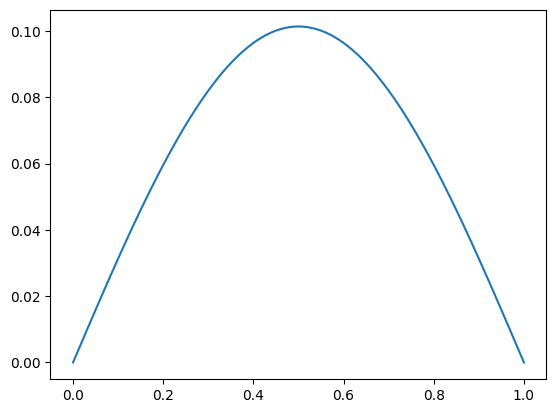
\includegraphics[width=0.6\linewidth]{Clase5_Practica3/difs_c5p3.png}
\end{figure}